\subsection{Diseño Orientado a Objetos}

\subsubsection{Ciclo de vida de una consulta}

El siguiente diagrama (figura \ref{fig:sequence_sinatra}) muestra la interacci\'on en los distintos componentes de la aplicaciones.

La primera interacci\'on es el request de la p\'agina principal index.html, que es la interfaz de usuario del prototipo, y contiene los formularios de b\'usqueda. El usuario hace un request tipo GET de la p\'agina, el cual es atendido por el componente Sinatra. Este \'ultimo tiene una ruta registrada que indica que este tipo de request debe ser atendido directamente por el componente HAML (pasand por par\'ametro el nombre del recurso solicitado). El componente HAML reconstruye el contenido html en base al recurso indicado, y lo devuelve a Sinatra para ser enviado al usuario.

La segunda interacci\'on es el request de resultados de b\'usqueda. El usuario hace un request tipo GET del recurso search, pasando los par\'ametros de b\'usqueda, el cual es atendido por el componente Sinatra. Este \'ultimo tiene una ruta registrada que indica que este tipo de request debe ser atendido primero por el componente PrecioJustoController, el cual valida los par\'ametros, crea los filtros (a trav\'es de FiltersFactory), y hace el llamado al componente PrecioJustoService para procesar la b\'usqueda. Una vez resuelta la b\'usqueda, se llama al componente HAML para que construya el html con los resultados, el cual se pasa al componente Sinatra para ser enviado al usuario.

Los componentes de PrecioJustoService y de FiltesFactory ser\'an explicados con mayor profundidad en las sucesivas secciones.

\begin{figure}[h]
\centerline{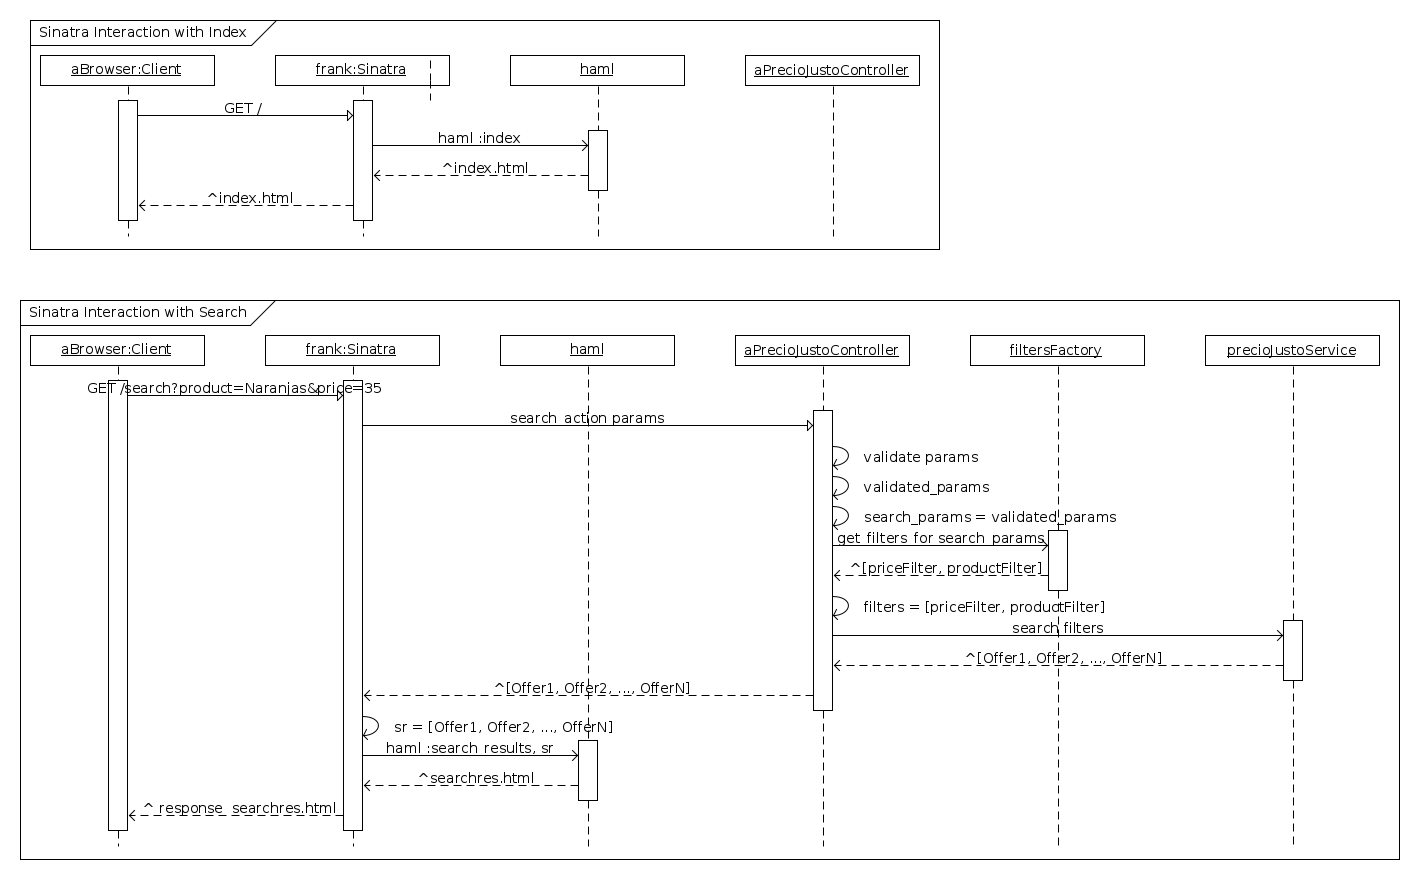
\includegraphics[width=0.6\paperwidth]{./imgs/sequence_diagram_sinatra.png}}
\caption{Diagrama de secuencia de sinatra}
\label{fig:sequence_sinatra}
\end{figure}

\subsubsection{B\'usqueda de ofertas}
\begin{figure}[h]
\centerline{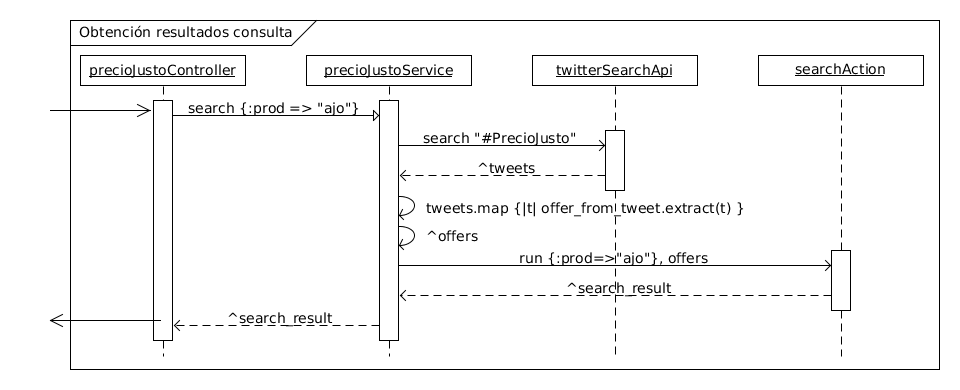
\includegraphics[width=0.6\paperwidth]{./imgs/sequence_searchAction.png}}
\caption{Diagrama de secuencia de procesamiento b\'usqueda}
\label{fig:sequence_sinatra}
\end{figure}

Mostramos en el diagrama de secuencia que se encuentra a continuaci\'on c\'omo se procesa una consulta desde $elPrecioJustoController$ hasta las capas inferiores de aplicaci\'on.
El procesamiento de una b\'usqueda luego de ser atendida por Sinatra, se delega en $elPrecioJustoController$, este delega la b\'usqueda en $elPrecioJustoService$. Veremos en las subsiguientes secciones, c\'omo  se generan los servicios por lo pronto veamos las delegaciones y como se procesan las b\'usquedas.

Por un lado observemos que el servicio toma como entrada un diccionario de filtros clave, valor. Estos son los filtros que aplicar\'a a cada oferta.
En un primer paso obtiene los tweets cuyo hashtag coincide con $\#PrecioJusto$. Luego, se transforma cada tweet en una oferta. Esto \'ultimo es delegado en el responsable de esta tarea $offer_from_tweet$.

A partir de este momento se tiene por un lado, un iterador de las ofertas y por otro, los filtros a aplicar cada una. El encargado de aplicar unos a otros es el $searchAction$ que por cada oferta aplica el filtro. Este resultado parcial es pasado por cada filtro hasta retornar la lista de ofertas filtradas de acuerdo a todos los criterios de b\'usqueda.




\subsubsection{Factory de servicios}
Twitter expone varias APIs para la obtenci\'on de tweets; las dos m\'as relevantes son la API de Streaming y la API de Search. Estas dos APIs tiene comportamientos muy diferentes.

\begin{itemize}
\item Streaming: requiere establecer una conexi\'on persistente HTTP (Chunked Encoding, Streaming), usando autenticaci\'on (OAuth). Devuelve los tweets que contienen los t\'erminos buscados, en tiempo real, o sea que los resultados ya devueltos no vuelven a aparecer. No impone l\'imites a las b\'usquedas y cantidad de conexiones, aunque s\'i tiene pol\'iticas para las reconexiones.
\item Search: recibe, procesa y responde cada request en su totalidad, finalizando en el request en el momento, sin requerir autenticaci\'on. Tiene un l\'imite para la cantidad de resultados devueltos, y para la antig\"uedad de \'estos; adem\'as impone l\'imites para la cantidad de requests.
\end{itemize}

En el caso de la API de Streaming, una posibilidad de uso es mantener una o varias b\'usquedas del maestro de productos y as\'i ir actualizando un repositorio interno/intermedio, el cual es utilizado para responder a las b\'usquedas de los usuarios de la aplicaci\'on.

Para la API de Search, un uso posible es resolver las b\'usquedas de los usuarios de la aplicaci\'on directamente contra \'esta.

En nuestro caso, implementamos ambas formas de trabajar con los tweets, asegur\'andonos que el intercambio de una por otra sea transparente: desde el lado de clientes de la b\'uqueda de ofertas de El Precio de Justo mantienen la misma interfaz.

Para esto \'ultimo decidimos utlizar el patr\'on de \texttt{abstract factory} con dos
implementaciones, una online (contra Twitter - API Search) y otra offline (contra un repositorio intermedio - API Streaming). Cada una de estas implementaciones nos permiten crear la clase de servicio apropiada (la clase que encapsula la l\'ogica de la aplicaci\'on), los filtros permitidos y la implementaci\'on espec\'ifica de \'estos.

\begin{figure}[h]
\centerline{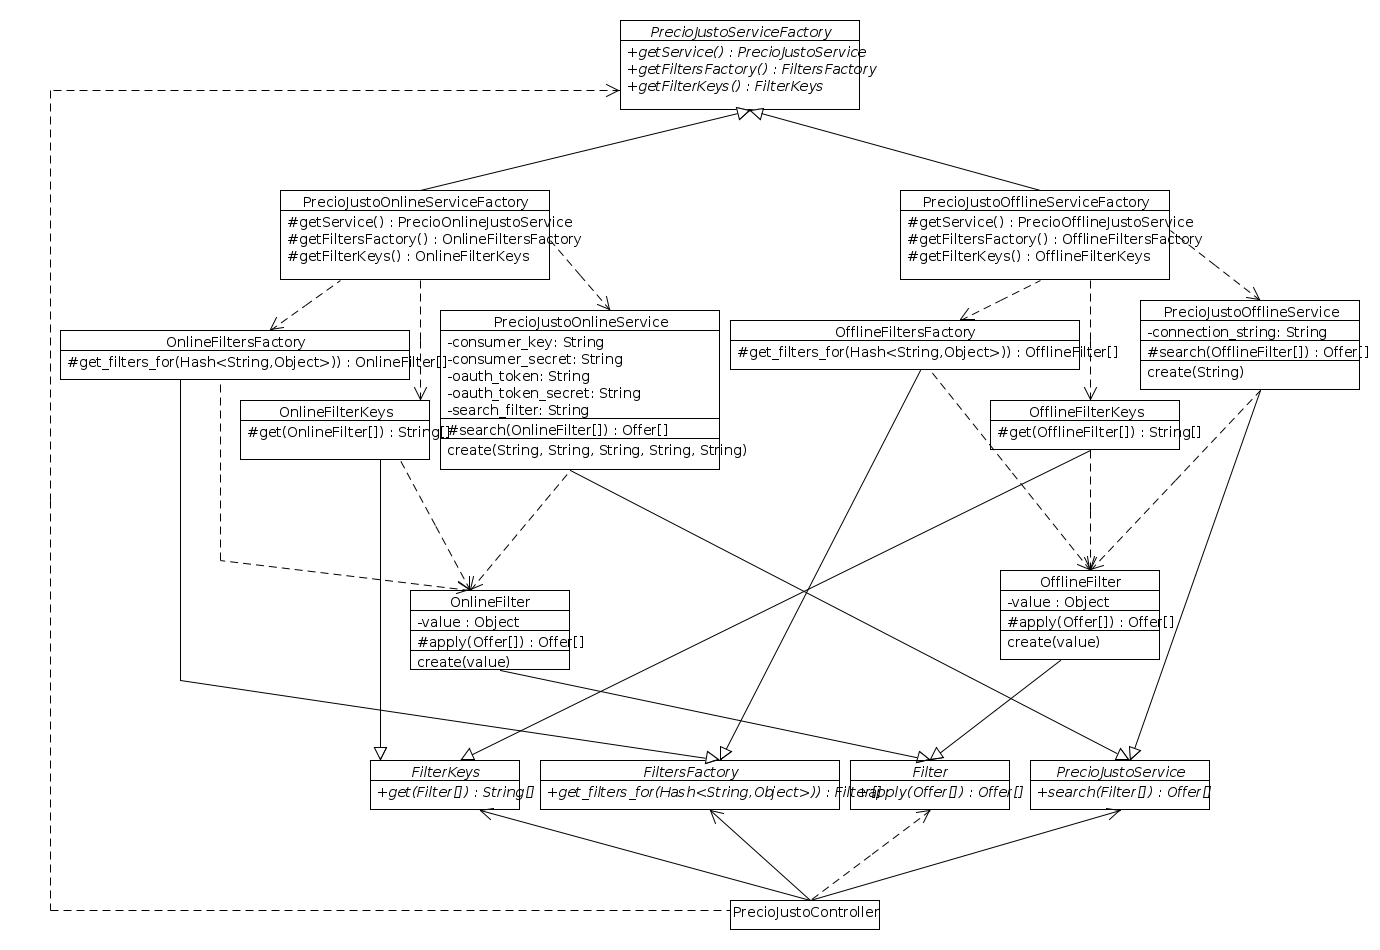
\includegraphics[width=0.44\paperwidth]{./imgs/class_diagram_service_factory_v2.png}}
\caption{Diagrama de clases de creaci\'on de servicios}
\label{fig:class_service_factory} 
\end{figure}

Esto \'ultimo puede verse en la figura \ref{fig:class_service_factory}. La clase abstracta PrecioJustoServiceFactory declara los m\'etodos getService, que devueve el tipo PrecioJustoService, getFiltersFactory, que devuelve el tipo FiltersFactory, y getFilterKeys, que devuelve el tipo FilterKeys. A su vez tenemos ambas familias de clases concretas, Online y Offline, que implementan los tipos definidos  previamente.

Los tipos de FilterKeys y FiltersFactory (y Filters), son utilizados por la clase de PrecioJustoController para traducir los filtros recibidos en los requests de usuario a filtros que sabe utilizar la implementaci\'on de PrecioJustoService (este tema se ver\'a en mayor detalle en el pr\'oximo punto).

Las clases de PrecioJustoOnlineService y PrecioJustoOfflineService implementan el tipo PrecioJustoService, y encapsulan la l\'ogica para resolver las b\'usquedas (accediendo directamente a Twitter en el primer caso, y accediendo a un repositorio interno en el segundo).


\subsubsection{Filtros}

Dado que el filtrado de los tweets de las ofertas b\'uscadas se realizan de distinta manera, los filtros si bien deber\'an proveer las misma funcionalidad son implementativamente distintos.

En un caso filtrar\'an las ofertas que se vayan obtienendo de twitter en vivo y en el otro caso se realizar\'a un b\'usqueda sobre el motor de base de datos.

Los filtros modelados son por producto, precio y ubicaci\'on, si bien es posible extenderlos.

Esto puede verse en el diagrama de la figura \ref{fig:class_filter_factory}. 

\begin{figure}[h]
\centerline{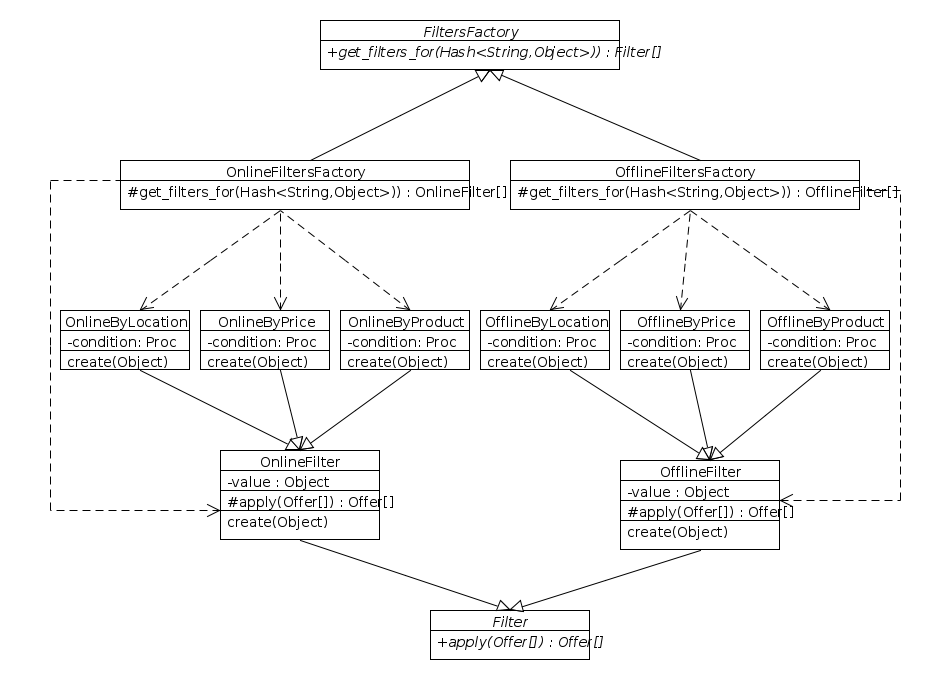
\includegraphics[width=0.6\paperwidth]{./imgs/class_diagram_filters_factory.png}}
\caption{Diagrama de clases de creaci\'on de filtros}
\label{fig:class_filter_factory} 
\end{figure}

\subsubsection{Extracci\'on de datos de un tweet}
La extracci\'on de las informaci\'on de las ofertas que se encuentra en los tweets se realiza mediante objetos de la clase \texttt{OfferFromTweetExtractor} (clase abstracta).
Para la demostraci\'on realizamos una implementaci\'on que extrae la informaci\'on mediante expresiones regulares para cada pedazo de informaci\'on dentro del texto, salvo para la geolocalizaci\'on del tweet.
Si bien no est\'a implementado para la demo, es deseable delegar la creaci\'on de las instancias de \texttt{Offer}. Para ello pensamos realizar mediante un \texttt{OfferBuilder}, la tarea del mismo ser\'ia realizar las acciones necesarias para crear una nueva instanacia. Ver diagrama de clases en la figura \ref{fig:class_parsing}

La idea es que cada pedazo de informaci\'on genere una instancia de un objeto polim\'orfico de la informaci\'on que modela (ej: el precio, producto, unidad).
Cuando nos refer\'imos a objetos polim\'orficos, queremos decir que la informaci\'on podr\'ia no poder generar un objeto v\'alido y queremos que resulte transparente para los objetos con los que interactuan con dicho objeto (la idea es poder implementar \texttt{Null Object Pattern})

\begin{figure}[h]
\centerline{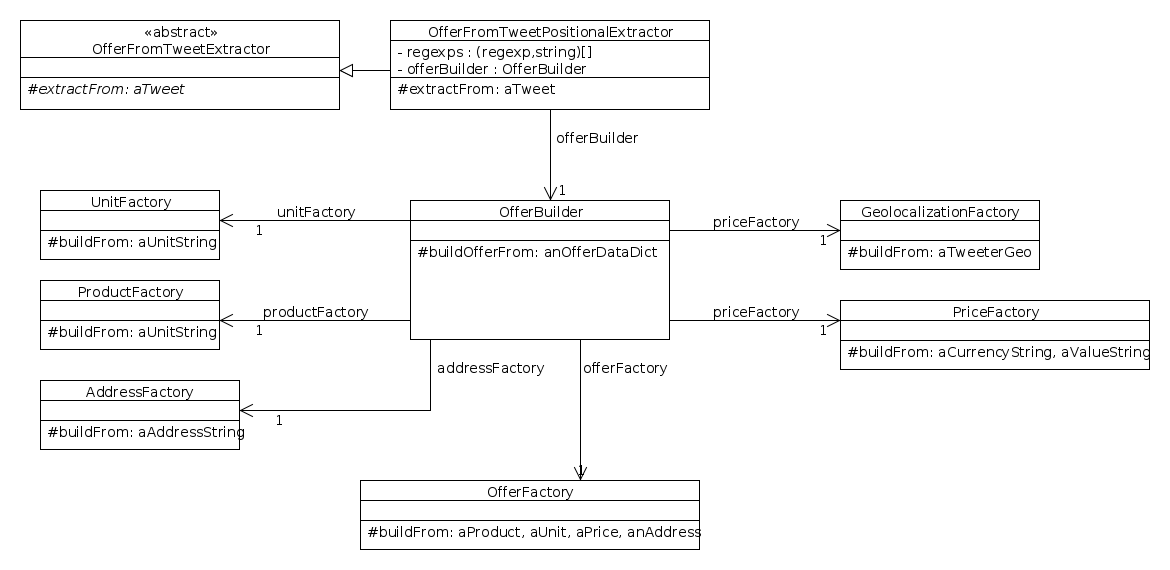
\includegraphics[width=0.9\paperwidth]{./imgs/class_diagram_parsing.png}}
\caption{Diagrama de clases de extraccion datos de tweet}
\label{fig:class_parsing}
\end{figure}

Respecto a la secuencia

\begin{figure}[h]
\centerline{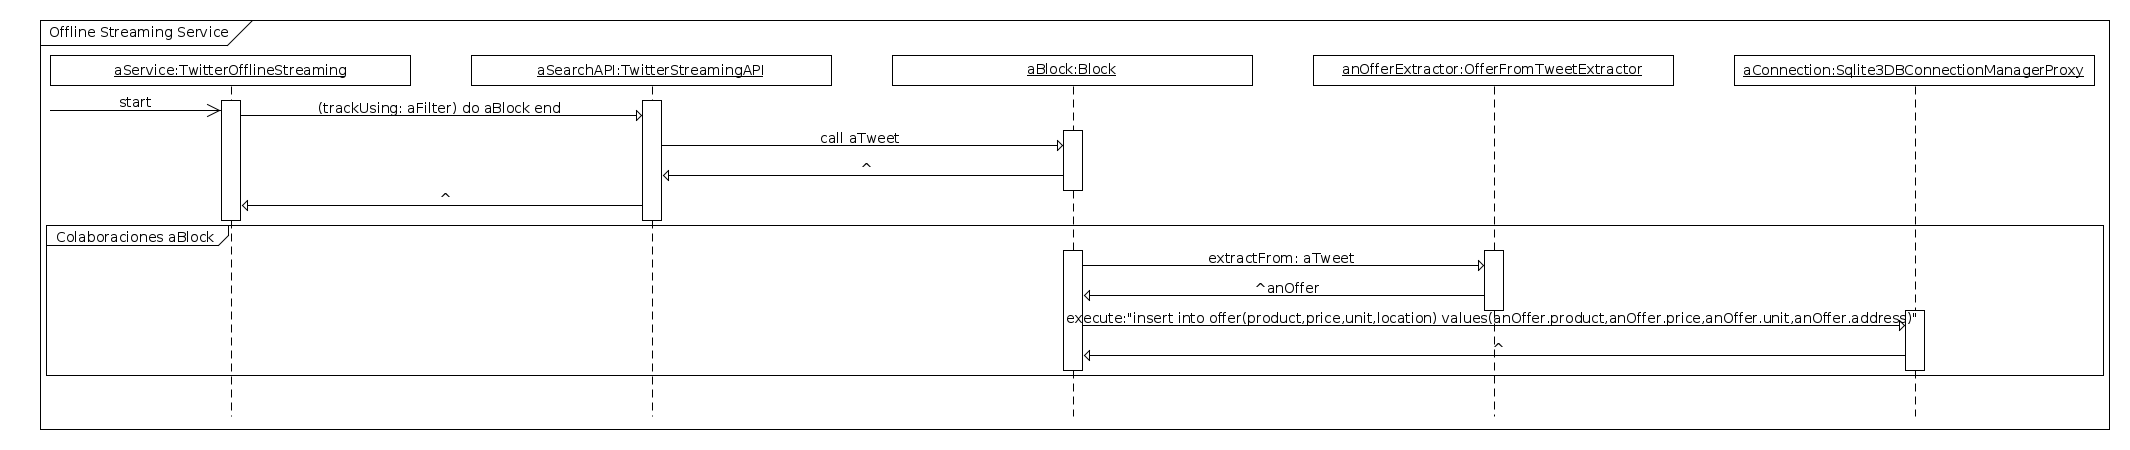
\includegraphics[keepaspectratio,width=\paperwidth,height=\paperheight,keepaspectratio,angle=90]{./imgs/sequence_diagram_offline_extraction.png}}
\caption{Diagrama de secuencia de obtención de ofertas a partir de tweets del servicio offline}
\label{fig:sequence_diagram_offline_extraction}
\end{figure}

\begin{figure}[h]
\centerline{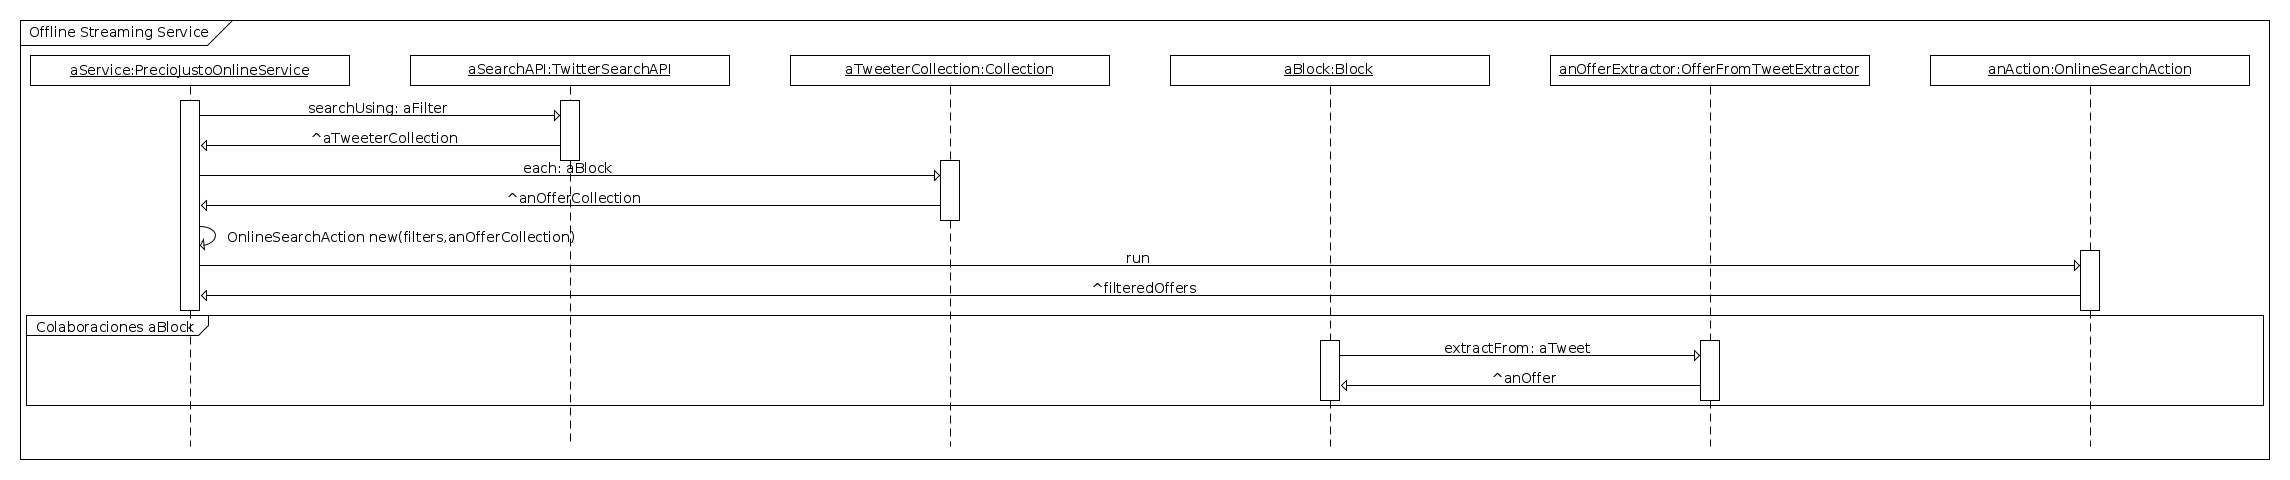
\includegraphics[keepaspectratio,width=\paperwidth,height=\paperheight,keepaspectratio,angle=90]{./imgs/sequence_diagram_online_extraction.png}}
\caption{Diagrama de secuencia de obtención de ofertas a partir de tweets del servicio online}
\label{fig:sequence_diagram_offline_extraction}
\end{figure}


\begin{figure}[h]
\centerline{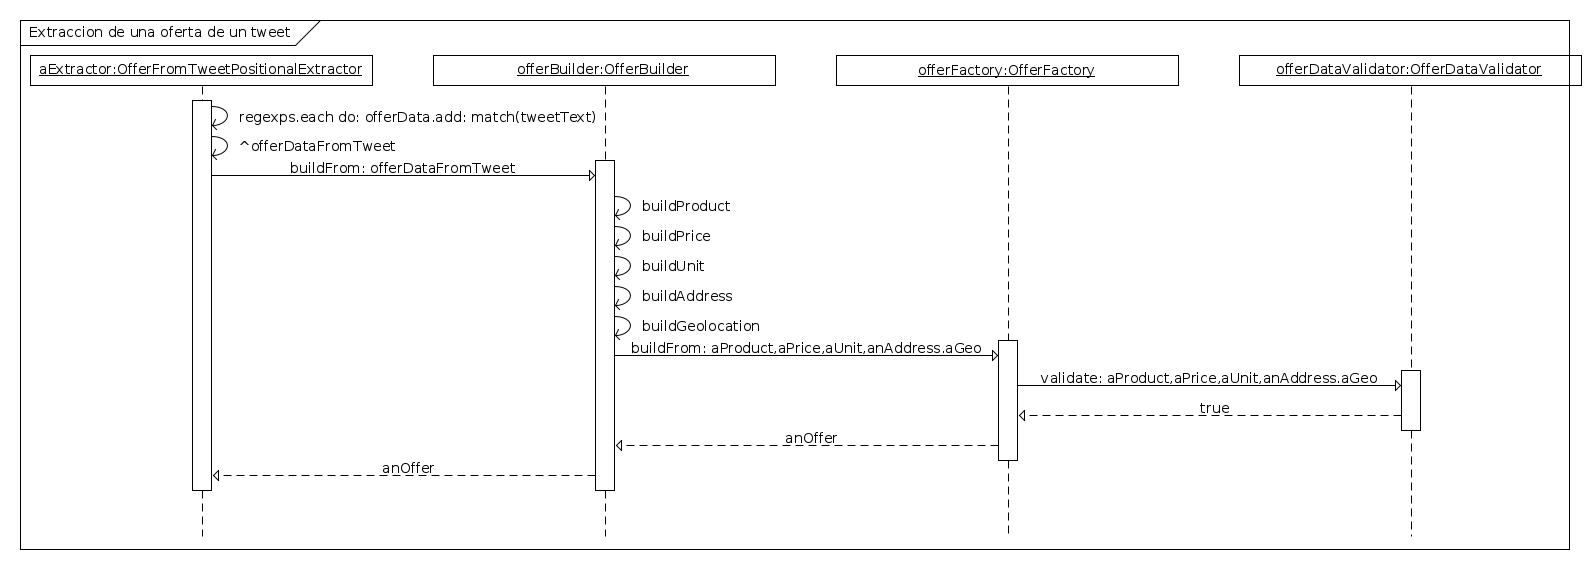
\includegraphics[width=0.9\paperwidth]{./imgs/sequence_diagram_parsing.png}}
\caption{Diagrama de secuencia de extraccion de datos de tweet}
\label{fig:secuence_parsing}
\end{figure}

\subsubsection{Servicio Online}
En este caso la clase PrecioJustoOnlineService encapsula la l\'ogica de la aplicaci\'on utilizando como fuente de informaci\'on las b\'usquedas directas en \texttt{Twitter} mediante la \texttt{API} de \texttt{Search}.
Para aplicar los filtros utiliza las clases derivadas de \texttt{OnlineFilter} y utiliza \texttt{OfferFromTweetPositionalExtractor} para la extracci\'on de las ofertas.

\begin{figure}[h]
\centerline{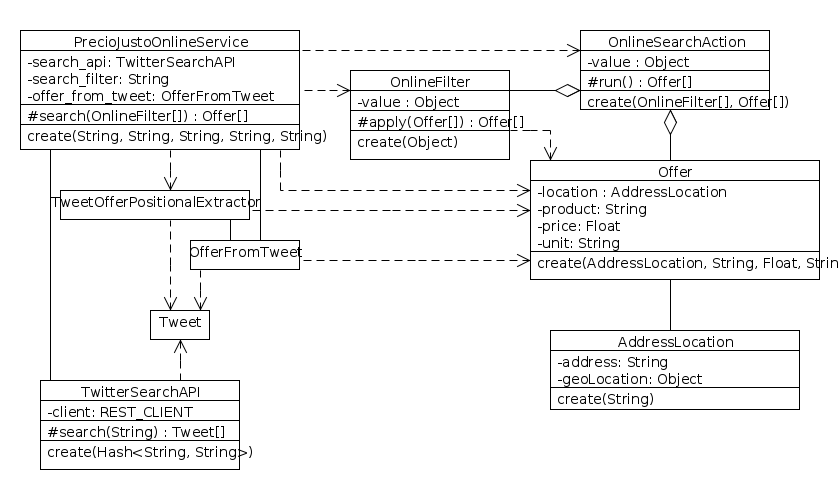
\includegraphics[width=0.9\paperwidth]{./imgs/class_diagram_online_service.png}}
\caption{Diagrama de clases de servicio online}
\label{fig:class_online_service}
\end{figure}

\subsubsection{Servicio Offline}

\textbf{PrecioJustoOfflineService}\\

En este caso la clase \texttt{PrecioJustoOfflineService} encapsula la l\'ogica de la aplicaci\'on utilizando como fuente de informaci\'on una base de datos \texttt{SQLite3}. La cual es alimentada mediante un servicio independiente.

Para aplicar los filtros utiliza las clases derivadas de \texttt{OfflineFilter}. Las ofertas
ya fueron parseadas antes de ser insertadas en la base de datos.

\begin{figure}[h]
\centerline{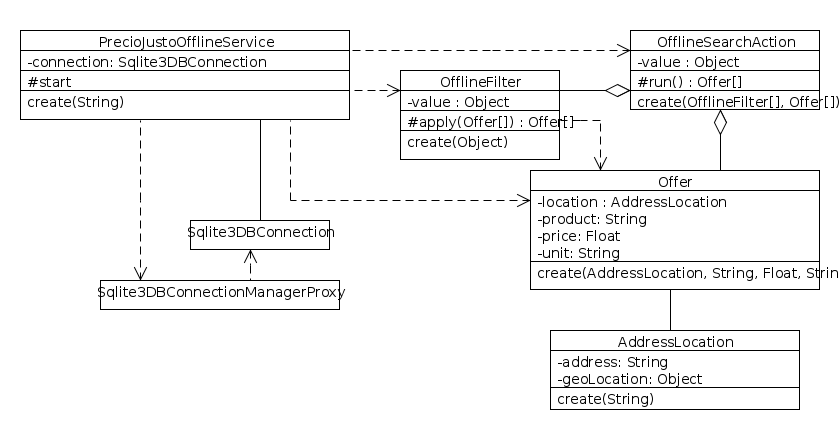
\includegraphics[width=0.9\paperwidth]{./imgs/class_diagram_offline_service.png}}
\caption{Diagrama de clases de servicio offline}
\label{fig:class_offline_service}
\end{figure}

\textbf{Servicio de Streaming}\\

Este proceso independiente utiliza la \texttt{API} de \texttt{Streaming} de \texttt{Twitter} para obtener las ofertas y persistirlas en la base de datos.

Para la extracci\'on de las ofertas de los tweets utiliza el extractor \texttt{OfferFromTweetPositionalExtractor}.

\begin{figure}[h]
\centerline{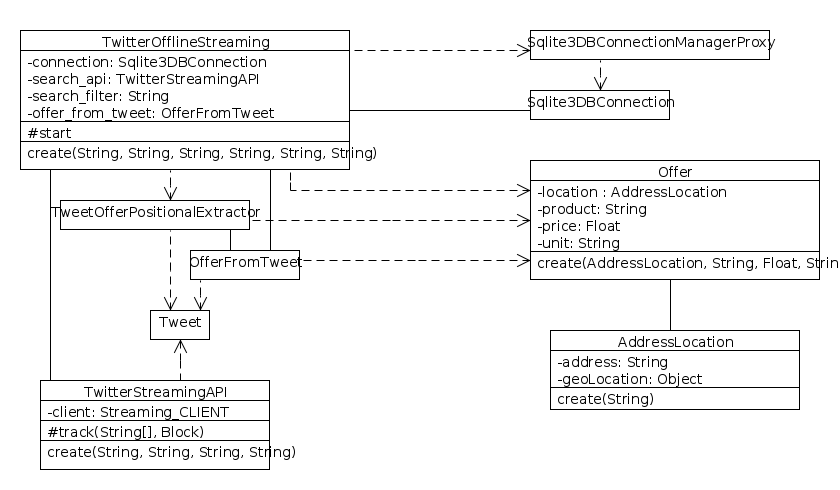
\includegraphics[width=0.9\paperwidth]{./imgs/class_diagram_offline_streaming.png}}
\caption{Diagrama de clases de streaming de twitter}
\label{fig:class_offline_streaming}
\end{figure}

\textbf{Cliente/Servidor SQLite3}\\

Dado la base de datos \texttt{SQLite3} es un archivo, el mismo se bloquea al accederlo
directamente. Para evitar esto generamos un proceso independiente que es el \'unico que bloque el archivo, pero expone mediante \texttt{DRB (remoting)} la conexi\'on a esta base para poder ser usada concurrentemente por distintos proceso.

\begin{figure}[h]
\centerline{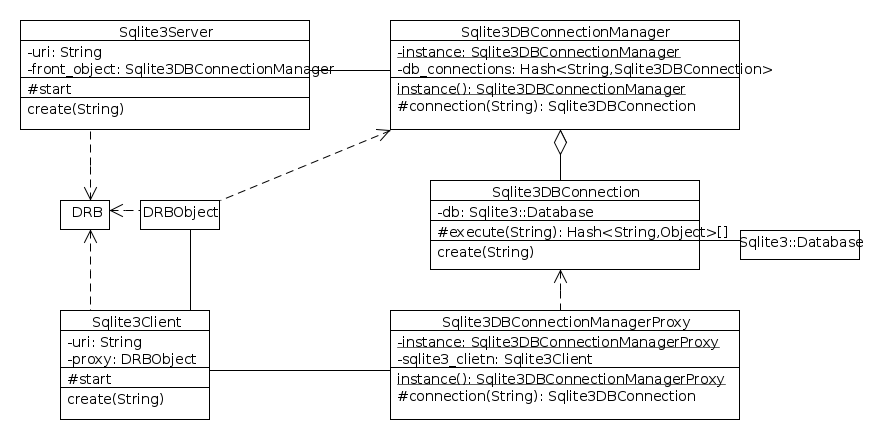
\includegraphics[width=0.9\paperwidth]{./imgs/class_diagram_sqlite3_client_server.png}}
\caption{Diagrama de clases de BD SQLite3}
\label{fig:class_sqlite3_client_server}
\end{figure}

\textbf{Ofertas y colaboradores}

El siguiente diagramas muestra el modelo de las ofertas (\texttt{Offer}) y sus colaboradores. Dichos colaboradores no est\'an modelados en la demostraci\'on.
El siguiente diagramas muestra la idea de creaci\'on de los distintos objetos
con la idea de poder generar objetos no v\'alidos polim\'orficos a los v\'alidos.

\begin{figure}[h]
\centerline{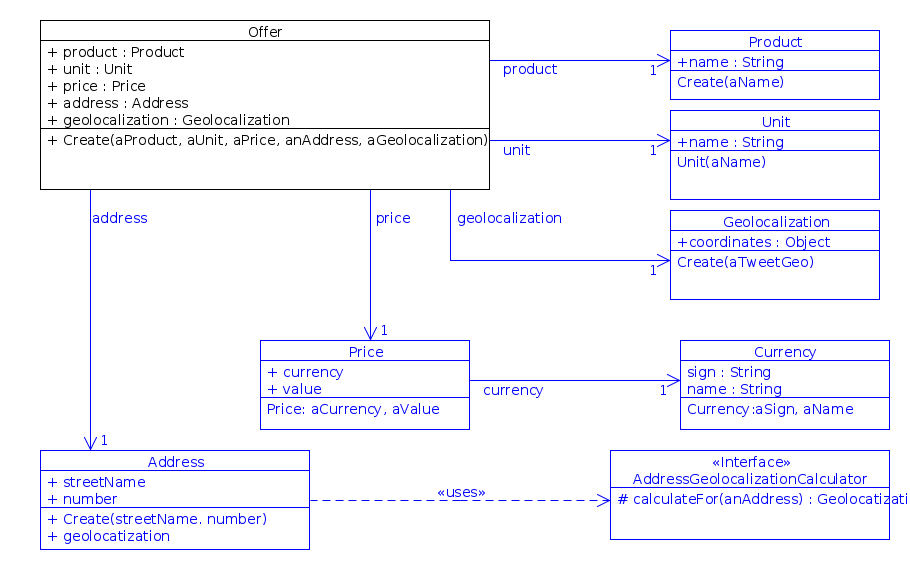
\includegraphics[width=0.9\paperwidth]{./imgs/class_diagram_offer.png}}
\caption{Diagrama de clases de offer y colaboradores}
\label{fig:class_offer}
\end{figure}

\begin{figure}[h]
\centerline{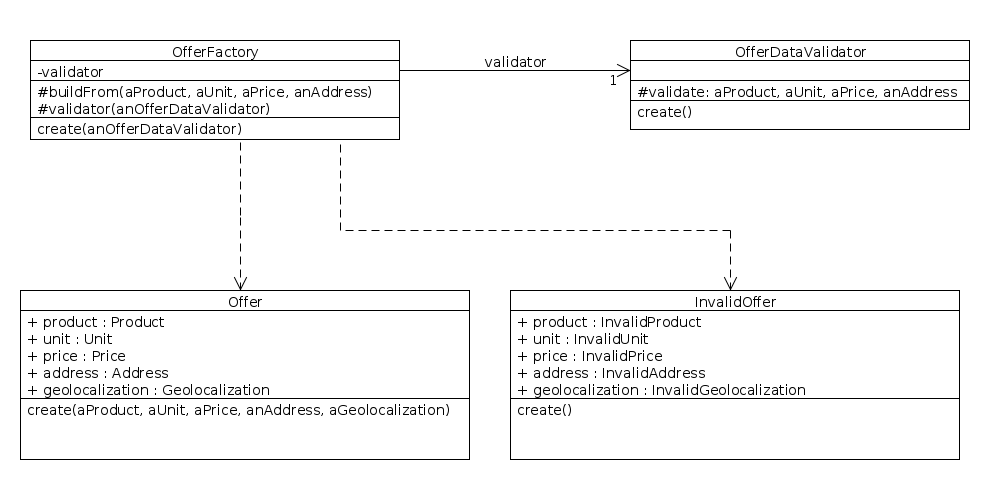
\includegraphics[width=0.9\paperwidth]{./imgs/class_diagram_Offer_Factory.png}}
\caption{Diagrama de clases de creaci\'on de offer}
\label{fig:class_Offer_Factory}
\end{figure}

